% Options for packages loaded elsewhere
\PassOptionsToPackage{unicode}{hyperref}
\PassOptionsToPackage{hyphens}{url}
\PassOptionsToPackage{dvipsnames,svgnames,x11names}{xcolor}
%
\documentclass[
  letterpaper,
  DIV=11,
  numbers=noendperiod]{scrartcl}

\usepackage{amsmath,amssymb}
\usepackage{iftex}
\ifPDFTeX
  \usepackage[T1]{fontenc}
  \usepackage[utf8]{inputenc}
  \usepackage{textcomp} % provide euro and other symbols
\else % if luatex or xetex
  \usepackage{unicode-math}
  \defaultfontfeatures{Scale=MatchLowercase}
  \defaultfontfeatures[\rmfamily]{Ligatures=TeX,Scale=1}
\fi
\usepackage{lmodern}
\ifPDFTeX\else  
    % xetex/luatex font selection
\fi
% Use upquote if available, for straight quotes in verbatim environments
\IfFileExists{upquote.sty}{\usepackage{upquote}}{}
\IfFileExists{microtype.sty}{% use microtype if available
  \usepackage[]{microtype}
  \UseMicrotypeSet[protrusion]{basicmath} % disable protrusion for tt fonts
}{}
\makeatletter
\@ifundefined{KOMAClassName}{% if non-KOMA class
  \IfFileExists{parskip.sty}{%
    \usepackage{parskip}
  }{% else
    \setlength{\parindent}{0pt}
    \setlength{\parskip}{6pt plus 2pt minus 1pt}}
}{% if KOMA class
  \KOMAoptions{parskip=half}}
\makeatother
\usepackage{xcolor}
\setlength{\emergencystretch}{3em} % prevent overfull lines
\setcounter{secnumdepth}{-\maxdimen} % remove section numbering
% Make \paragraph and \subparagraph free-standing
\makeatletter
\ifx\paragraph\undefined\else
  \let\oldparagraph\paragraph
  \renewcommand{\paragraph}{
    \@ifstar
      \xxxParagraphStar
      \xxxParagraphNoStar
  }
  \newcommand{\xxxParagraphStar}[1]{\oldparagraph*{#1}\mbox{}}
  \newcommand{\xxxParagraphNoStar}[1]{\oldparagraph{#1}\mbox{}}
\fi
\ifx\subparagraph\undefined\else
  \let\oldsubparagraph\subparagraph
  \renewcommand{\subparagraph}{
    \@ifstar
      \xxxSubParagraphStar
      \xxxSubParagraphNoStar
  }
  \newcommand{\xxxSubParagraphStar}[1]{\oldsubparagraph*{#1}\mbox{}}
  \newcommand{\xxxSubParagraphNoStar}[1]{\oldsubparagraph{#1}\mbox{}}
\fi
\makeatother


\providecommand{\tightlist}{%
  \setlength{\itemsep}{0pt}\setlength{\parskip}{0pt}}\usepackage{longtable,booktabs,array}
\usepackage{calc} % for calculating minipage widths
% Correct order of tables after \paragraph or \subparagraph
\usepackage{etoolbox}
\makeatletter
\patchcmd\longtable{\par}{\if@noskipsec\mbox{}\fi\par}{}{}
\makeatother
% Allow footnotes in longtable head/foot
\IfFileExists{footnotehyper.sty}{\usepackage{footnotehyper}}{\usepackage{footnote}}
\makesavenoteenv{longtable}
\usepackage{graphicx}
\makeatletter
\def\maxwidth{\ifdim\Gin@nat@width>\linewidth\linewidth\else\Gin@nat@width\fi}
\def\maxheight{\ifdim\Gin@nat@height>\textheight\textheight\else\Gin@nat@height\fi}
\makeatother
% Scale images if necessary, so that they will not overflow the page
% margins by default, and it is still possible to overwrite the defaults
% using explicit options in \includegraphics[width, height, ...]{}
\setkeys{Gin}{width=\maxwidth,height=\maxheight,keepaspectratio}
% Set default figure placement to htbp
\makeatletter
\def\fps@figure{htbp}
\makeatother
% definitions for citeproc citations
\NewDocumentCommand\citeproctext{}{}
\NewDocumentCommand\citeproc{mm}{%
  \begingroup\def\citeproctext{#2}\cite{#1}\endgroup}
\makeatletter
 % allow citations to break across lines
 \let\@cite@ofmt\@firstofone
 % avoid brackets around text for \cite:
 \def\@biblabel#1{}
 \def\@cite#1#2{{#1\if@tempswa , #2\fi}}
\makeatother
\newlength{\cslhangindent}
\setlength{\cslhangindent}{1.5em}
\newlength{\csllabelwidth}
\setlength{\csllabelwidth}{3em}
\newenvironment{CSLReferences}[2] % #1 hanging-indent, #2 entry-spacing
 {\begin{list}{}{%
  \setlength{\itemindent}{0pt}
  \setlength{\leftmargin}{0pt}
  \setlength{\parsep}{0pt}
  % turn on hanging indent if param 1 is 1
  \ifodd #1
   \setlength{\leftmargin}{\cslhangindent}
   \setlength{\itemindent}{-1\cslhangindent}
  \fi
  % set entry spacing
  \setlength{\itemsep}{#2\baselineskip}}}
 {\end{list}}
\usepackage{calc}
\newcommand{\CSLBlock}[1]{\hfill\break\parbox[t]{\linewidth}{\strut\ignorespaces#1\strut}}
\newcommand{\CSLLeftMargin}[1]{\parbox[t]{\csllabelwidth}{\strut#1\strut}}
\newcommand{\CSLRightInline}[1]{\parbox[t]{\linewidth - \csllabelwidth}{\strut#1\strut}}
\newcommand{\CSLIndent}[1]{\hspace{\cslhangindent}#1}

\KOMAoption{captions}{tableheading}
\makeatletter
\@ifpackageloaded{caption}{}{\usepackage{caption}}
\AtBeginDocument{%
\ifdefined\contentsname
  \renewcommand*\contentsname{Table of contents}
\else
  \newcommand\contentsname{Table of contents}
\fi
\ifdefined\listfigurename
  \renewcommand*\listfigurename{List of Figures}
\else
  \newcommand\listfigurename{List of Figures}
\fi
\ifdefined\listtablename
  \renewcommand*\listtablename{List of Tables}
\else
  \newcommand\listtablename{List of Tables}
\fi
\ifdefined\figurename
  \renewcommand*\figurename{Figure}
\else
  \newcommand\figurename{Figure}
\fi
\ifdefined\tablename
  \renewcommand*\tablename{Table}
\else
  \newcommand\tablename{Table}
\fi
}
\@ifpackageloaded{float}{}{\usepackage{float}}
\floatstyle{ruled}
\@ifundefined{c@chapter}{\newfloat{codelisting}{h}{lop}}{\newfloat{codelisting}{h}{lop}[chapter]}
\floatname{codelisting}{Listing}
\newcommand*\listoflistings{\listof{codelisting}{List of Listings}}
\makeatother
\makeatletter
\makeatother
\makeatletter
\@ifpackageloaded{caption}{}{\usepackage{caption}}
\@ifpackageloaded{subcaption}{}{\usepackage{subcaption}}
\makeatother

\ifLuaTeX
  \usepackage{selnolig}  % disable illegal ligatures
\fi
\usepackage{bookmark}

\IfFileExists{xurl.sty}{\usepackage{xurl}}{} % add URL line breaks if available
\urlstyle{same} % disable monospaced font for URLs
\hypersetup{
  pdftitle={World Development Indicators},
  pdfauthor={Emma Carrier},
  colorlinks=true,
  linkcolor={blue},
  filecolor={Maroon},
  citecolor={Blue},
  urlcolor={Blue},
  pdfcreator={LaTeX via pandoc}}


\title{World Development Indicators}
\author{Emma Carrier}
\date{2024-10-09}

\begin{document}
\maketitle


\subsection{Introduction}\label{introduction}

\section{GDP per Capita}\label{gdp-per-capita}

GDP per capita is a country's GDP divided by its total population
(Worldometer 2022). From the 203 countries with data on GDP per capita,
the mean is \$20345.71. The GDP per capita between different countries
vary greatly, with the maximum being \$240862.18 and the minimum being
\$259.03

\begin{verbatim}
count       203.000000
mean      20345.707649
std       31308.942225
min         259.025031
25%        2570.563284
50%        7587.588173
75%       25982.630050
max      240862.182448
Name: gdp_per_capita, dtype: float64
\end{verbatim}

\section{Inflation Rate}\label{inflation-rate}

The inflation rate in a country is the increase in prices over a given
period of time (Oner n.d.). The average inflation rate in th 169
observed countries is 12.5\%. Some countries have an inflation rate in
the negatives, with the minimum value in this dataset being -6.69\%

\begin{verbatim}
count    169.000000
mean      12.493936
std       19.682433
min       -6.687321
25%        5.518129
50%        7.967574
75%       11.665567
max      171.205491
Name: inflation_rate, dtype: float64
\end{verbatim}

\section{Measles Immunization Rates}\label{measles-immunization-rates}

Measles is an extremely deadly disease that has affected many nations
for centuries. The rate at which the populations in a country are
vaccinated for measles is greatly important to the overall health of the
population. From the observed 193 countries, the average measles
vaccination rate is 83.85\%.

\begin{verbatim}
count    193.000000
mean      83.854922
std       15.996083
min        0.000000
25%       76.000000
50%       90.000000
75%       96.000000
max       99.000000
Name: measles_immunisation_rate, dtype: float64
\end{verbatim}

\section{GDP Growth Rate}\label{gdp-growth-rate}

The GDP growth rate measures how fast a country's economy is growing /
shrinking each year. This visualization compares a country's growth rate
and it's GDP per capita in the year 2022. From the graph, it appears
that many of the countries that have higher GDPs do not have either a
high or low GDP growth rate.

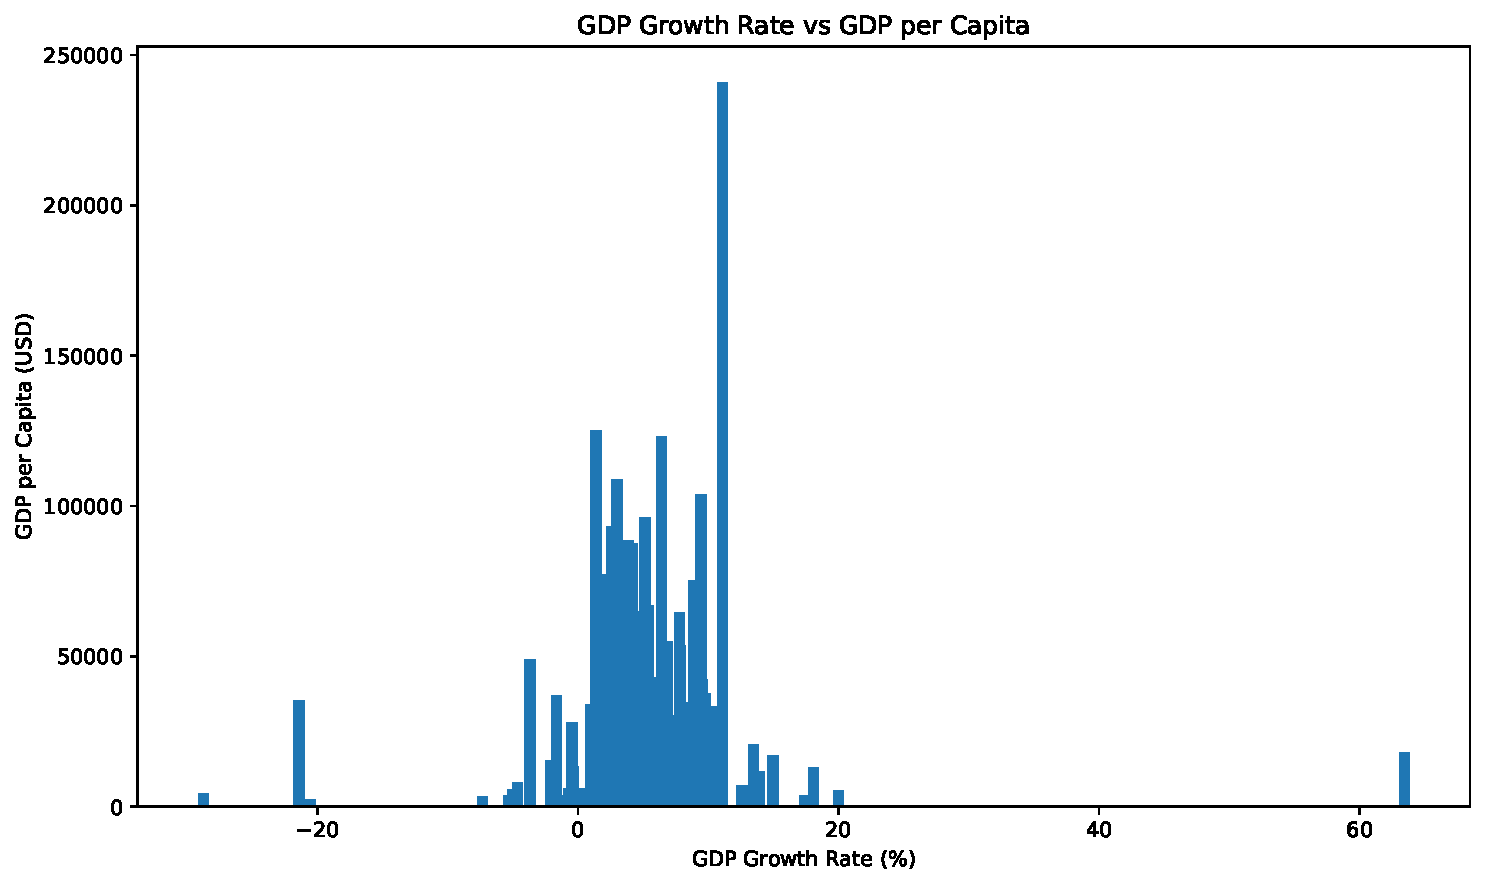
\includegraphics{assignment_05_files/figure-pdf/cell-6-output-1.pdf}

Figure 1: a bar chart showing the GDP Growth Rate vs GDP per Capita.
Source: (Bank 2024)

\section{Measles Immunisation Rate vs Life
Expectancy}\label{measles-immunisation-rate-vs-life-expectancy}

This graph compares the percentage of the popualtion in a country that
has received an immunisation from measles. According to the data,
countries that have a higher percentage of their population vaccinated
for measles, the average life expectancy is higher.

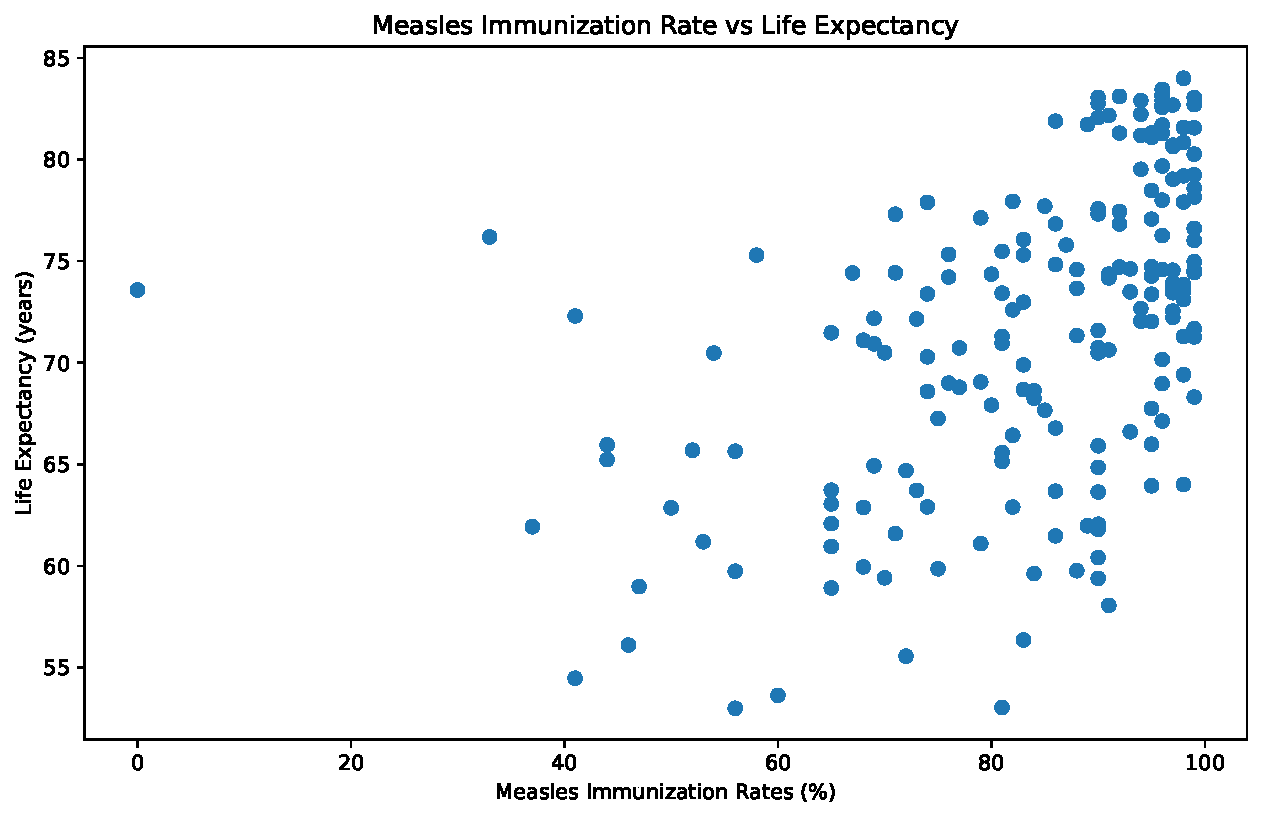
\includegraphics{assignment_05_files/figure-pdf/cell-7-output-1.pdf}

Figure 2: a scatter plot showing the Measles Immunization rate vs Life
Expectancy. Source: (Bank 2024)

\section{Key Findings and Statistics}\label{key-findings-and-statistics}

\begin{longtable}[]{@{}llll@{}}
\toprule\noalign{}
& measles\_immunisation\_rate & gdp\_growth\_rate & inflation\_rate \\
\midrule\noalign{}
\endhead
\bottomrule\noalign{}
\endlastfoot
count & 193.000000 & 202.000000 & 169.000000 \\
mean & 83.854922 & 4.368901 & 12.493936 \\
std & 15.996083 & 6.626811 & 19.682433 \\
min & 0.000000 & -28.758591 & -6.687321 \\
25\% & 76.000000 & 2.438593 & 5.518129 \\
50\% & 90.000000 & 4.204431 & 7.967574 \\
75\% & 96.000000 & 6.200000 & 11.665567 \\
max & 99.000000 & 63.439864 & 171.205491 \\
\end{longtable}

\phantomsection\label{refs}
\begin{CSLReferences}{1}{0}
\bibitem[\citeproctext]{ref-worldbank_wdi}
Bank, World. 2024. {``World Development Indicators.''}
\url{https://databank.worldbank.org/source/world-development-indicators}.

\bibitem[\citeproctext]{ref-oner_inflation}
Oner, Ceyda. n.d. {``Inflation: Prices on the Rise.''} \emph{Finance \&
Development: Back to Basics}, n.d., 30--31.
\url{https://www.imf.org/en/Publications/fandd/issues/Series/Back-to-Basics/Inflation}.

\bibitem[\citeproctext]{ref-worldometer_gdp}
Worldometer. 2022. {``GDP Per Capita by Country.''}
\url{https://www.worldometers.info/gdp/gdp-per-capita/}.

\end{CSLReferences}




\end{document}
